\raggedright
\section{Chapter 2: Single Variable Analyses}
\paragraph{Types of Variables}
\centering
Nominal \makebox[0pt][l]{(Cate)}\\
\makebox[0pt][r]{Meaningful Order\ }$\Downarrow$\\
Ordinal \makebox[0pt][l]{(Cate)}\\
\makebox[0pt][r]{Consistent Difference\ }$\Downarrow$\\
Discrete \makebox[0pt][l]{(Quant)}\\
\makebox[0pt][r]{(Uncountably) Infinite\ }$\Downarrow$\\
Continuous \makebox[0pt][l]{(Quant)}

\raggedright
\paragraph{Describing Data}
\textcolor{Bittersweet}{Continuous Variables:}
\begin{itemize}
	\item Cluster/Gap Intervals
	\item Suspected Outliers [Small/Large] ($z-score>3$)
	\item Modality
	\item Skewness
	\begin{enumerate}
		\item Symmetric \& Bell-Shaped: (Sensitive to Skew)
		\begin{itemize}
			\item Mean
			\item Var \& Std Dev
		\end{itemize}
		\item Highly Skewed: (Robust to Outliers)
		\begin{itemize}
			\item Median
			\item IQR (NOTE: Quantiles are non-unique)
		\end{itemize}
	\end{enumerate}
\end{itemize}
$\Rightarrow$ Continuous can be categorised!\\
\textcolor{Bittersweet}{Categorical (or Discrete) Variables:}
\begin{itemize}
	\item \% Proportion of Modal Category
	\item Special High/Low Categories
	\item (Ordinal) Apparent Trend in Proportions
\end{itemize}
\paragraph{Formulae and Results}
$\overline{X}=\frac{1}{n}\sum_{i=1}^nX_i$\\
$Var(X)=\frac{1}{n-1}\sum_{i-1}^n(X_i-\overline{X})^2$\\
\textcolor{Blue}{For $Y=aX+b$:}\\
$\overline{Y}=a\overline{X}+b$\\
$Var(Y)=a^2Var(X)$\\
$s_Y=\left|a\right|s_X$
\begin{Figure}
	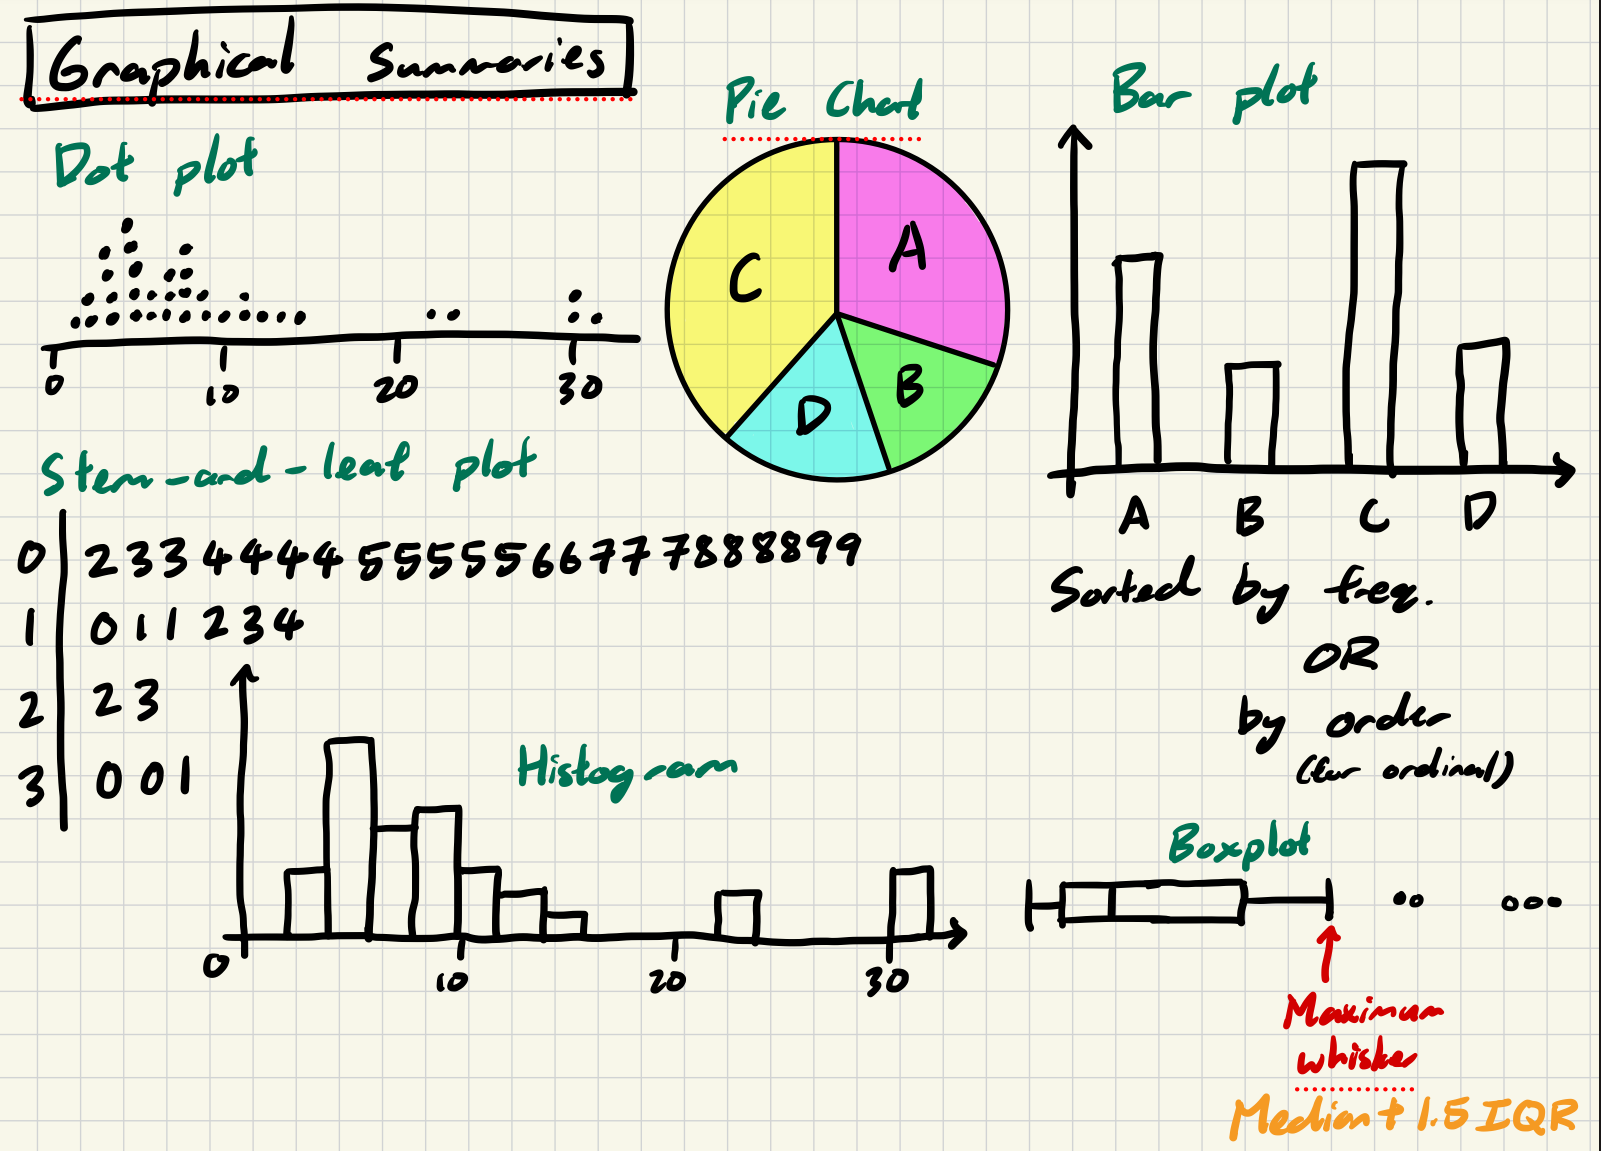
\includegraphics[width=\linewidth]{graphicalSummaries.png}
\end{Figure}